\documentclass[12pt]{article}
\usepackage[]{algorithm2e}
\usepackage{tikz}
\usepackage{ifthen}
% This first part of the file is called the PREAMBLE. It includes
% customizations and command definitions. The preamble is everything
% between \documentclass and \begin{document}.
\usepackage{amsthm}
\newtheorem{theorem}{Theorem}
\usepackage[margin=1in]{geometry}  % set the margins to 1in on all sides
\usepackage{graphicx}              % to include figures
\usepackage{amsmath}               % great math stuff
\usepackage{amsfonts}              % for blackboard bold, etc
\usepackage{amsthm}                % better theorem environments
\usepackage{changepage}
\usepackage{lipsum}                     % Dummytext
\usepackage{xargs}                      % Use more than one optional parameter in a new commands
 % Coloured text etc.
% 
\usepackage[colorinlistoftodos,prependcaption,textsize=tiny]{todonotes}
\newcommandx{\unsure}[2][1=]{\todo[linecolor=red,backgroundcolor=red!25,bordercolor=red,#1]{#2}}
\newcommandx{\change}[2][1=]{\todo[linecolor=blue,backgroundcolor=blue!25,bordercolor=blue,#1]{#2}}
\newcommandx{\info}[2][1=]{\todo[linecolor=OliveGreen,backgroundcolor=OliveGreen!25,bordercolor=OliveGreen,#1]{#2}}
\newcommandx{\improvement}[2][1=]{\todo[linecolor=Plum,backgroundcolor=Plum!25,bordercolor=Plum,#1]{#2}}
\newcommandx{\thiswillnotshow}[2][1=]{\todo[disable,#1]{#2}}
\newcommand{\blockmatrix}[9]{
	\draw[draw=#4,fill=#5] (0,0) rectangle( #1,#2);
	\ifthenelse{\equal{#6}{true}}
	{
		\draw[draw=#7,fill=#8] (0,#2) -- (#9,#2) -- ( #1,#9) -- ( #1,0) -- ( #1 - #9,0) -- (0,#2 -#9) -- cycle;
	}
	{}
	\draw ( #1/2, #2/2) node { #3};
}

% Quick implementation of a tikz right parenthesis
% \rightparen{width}
\newcommand{\rightparen}[1]{
	\begin{tikzpicture} 
	\draw (0,#1/2) arc (0:30:#1);
	\draw (0,#1/2) arc (0:-30:#1);
	\end{tikzpicture}%this comment is necessary
}

% Quick implementation of a tikz left parenthesis
% \leftparen{width}
\newcommand{\leftparen}[1]{
	\begin{tikzpicture} 
	\draw (0,#1/2) arc (180:150:#1);
	\draw (0,#1/2) arc (180:210:#1);
	\end{tikzpicture}%this comment is necessary
}

% Unframed block matrix, "m" prefix to match fbox, mbox
% \blockmatrix[r,g,b]{width}{height}{text}
\newcommand{\mblockmatrix}[4][none]{
	\begin{tikzpicture} 
	\ifthenelse{\equal{#1}{none}}
	{
		\blockmatrix{#2}{#3}{#4}{none}{none}{false}{none}{none}{0.0}
	}
	{
		\definecolor{fillcolor}{rgb}{#1}
		\blockmatrix{#2}{#3}{#4}{none}{fillcolor}{false}{none}{none}{0.0}
	}
	\end{tikzpicture}%this comment is necessary
}

% Framed block matrix
% \fblockmatrix[r,g,b]{width}{height}{text}
\newcommand{\fblockmatrix}[4][none]{
	\begin{tikzpicture} 
	\ifthenelse{\equal{#1}{none}}
	{
		\blockmatrix{#2}{#3}{#4}{black}{none}{false}{none}{none}{0.0}
	}
	{
		\definecolor{fillcolor}{rgb}{#1}
		\blockmatrix{#2}{#3}{#4}{black}{fillcolor}{false}{none}{none}{0.0}
	}
	\end{tikzpicture}%this comment is necessary
}

% Diagonal block matrix
% \dblockmatrix[r,g,b]{width}{height}{text}
\newcommand{\dblockmatrix}[4][none]{
	\begin{tikzpicture} 
	\ifthenelse{\equal{#1}{none}}
	{
		\blockmatrix{#2}{#3}{#4}{black}{none}{true}{black}{none}{0.35cm}
	}
	{
		\definecolor{fillcolor}{rgb}{#1}
		\blockmatrix{#2}{#3}{#4}{black}{none}{true}{black}{fillcolor}{0.35cm}
	}
	\end{tikzpicture}%this comment is necessary
}


% Diagonal block matrix, but exposes diagonal offset
% \diagonalblockmatrix[r,g,b]{width}{height}{text}
\newcommand{\diagonalblockmatrix}[5][none]{
	\begin{tikzpicture} 
	
	\ifthenelse{\equal{#1}{none}}
	{
		\blockmatrix{#2}{#3}{#4}{black}{none}{true}{black}{none}{#5}
	}
	{
		\definecolor{fillcolor}{rgb}{#1}
		\blockmatrix{#2}{#3}{#4}{black}{none}{true}{black}{fillcolor}{#5}
	}
	
	\end{tikzpicture}%necessary comment
}

\newcommand{\valignbox}[1]{
	\vtop{\null\hbox{#1}}% necessary comment
}

% a hack so that I don't have to worry about the number of columns or
% spaces between columns in the tabular environment
\newenvironment{blockmatrixtabular}
{% necessary comment
	\begin{tabular}{
			@{}l@{}l@{}l@{}l@{}l@{}l@{}l@{}l@{}l@{}l@{}l@{}l@{}l@{}l@{}l@{}l@{}l@{}l@{}l
			@{}l@{}l@{}l@{}l@{}l@{}l@{}l@{}l@{}l@{}l@{}l@{}l@{}l@{}l@{}l@{}l@{}l@{}l@{}l
			@{}l@{}l@{}l@{}l@{}l@{}l@{}l@{}l@{}l@{}l@{}l@{}l@{}l@{}l@{}l@{}l@{}l@{}l@{}l
			@{}
		}
	}
	{
	\end{tabular}%necessary comment
}
% various theorems, numbered by section

\newtheorem{thm}{Theorem}[section]
\newtheorem{lem}[thm]{Lemma}
\newtheorem{prop}[thm]{Proposition}
\newtheorem{cor}[thm]{Corollary}
\newtheorem{conj}[thm]{Conjecture}

\DeclareMathOperator{\id}{id}

\newcommand{\bd}[1]{\mathbf{#1}}  % for bolding symbols
\newcommand{\RR}{\mathbb{R}}      % for Real numbers
\newcommand{\ZZ}{\mathbb{Z}}      % for Integers
\newcommand{\col}[1]{\left[\begin{matrix} #1 \end{matrix} \right]}
\newcommand{\comb}[2]{\binom{#1^2 + #2^2}{#1+#2}}
\usepackage{graphicx}
\usepackage{csquotes}
\usepackage{lipsum}
\newcommand\tab[1][1cm]{\hspace*{#1}}

\begin{document}


\nocite{*}

\title{Hierarchical Topic Modeling and Visualization using Non-Negative Matrix Factorization 
	 \\ 
	Mathematics Senior Thesis}


\author{Ziv Epstein \\ 
	\texttt{ziv.epstein@pomona.edu}}

\maketitle
\newpage
\tableofcontents
\newpage
$$\color{green}\alpha E_{content}(\mathcal{C}, I) \color{black} +  \color{red} \beta E_{style}(\mathcal{S},I) = \color{orange}E_{overall}(\mathcal{S}, \mathcal{C}, I)$$
\section{Introduction to Topic Modeling}
With the vast amount of digital text being generated across the internet, methods for understanding and processing corpora of human language become necessary. Across mathematics and computer science, many techniques have been put forward that allow one to understand a body of text far too large to read herself. A successful method in this domain is \emph{topic modelling}, whereby semantically cohesive subgroups of words can be identified. In particular, let $\mathcal{C} = \{d_1,d_2,\cdots, d_n\}$ be a collection of documents with a vocabulary $\mathcal{V}$. A \emph{topic}  $t_i$ is a vector over the words in the vocabulary that represents a coherent high level notion in the corpus:
$$t_i = \{v^i_1, v^i_2, \cdots, v_m^i\}$$
where $m$ is the size of the vocabulary. Topic modelling offers a powerful tool for understanding large amounts of text because they can discover latent semantic structure within text. 

There are two primary techniques for learning these topics $t_i$. The first is LDA, a generative Bayesian statistical model which views each document $d_j$ as a mixture of various topics.
The second is non-negative matrix factorization, which aims to factor the document/word matrix into a document/topic and a topic/word matrix \cite{lee1999learning}. The focus of this thesis will be NNMF, because of its relation to linear algebra, and its deep visual and conceptual intuition. 
\todo{talk about high level structure of paper}


\section{Non Negative Matrix Factorization}
\subsection{How NNMF solves Topic Modeling}
Non-negative matrix factorization was first employed by Paatero and Tapper \cite{paatero1994positive} but was made popular by Lee and Seung \cite{lee1999learning} who suggested the importance of non-negative in human percetion and first linked it to topic modeling.

Given our $n$ documents with vocabulary $\mathcal{V}$ of size $m$, we construct a matrix $X \in \mathbb{R}^{n\times m}$ where $X_{i,j}$ is the number of occurences of word $j$ in document $i$. For a given inner dimension $k$, we seek to factor $X$ into two matrices $A$ and $S$ such that
$$X \approx AS$$
where $A \in \mathbb{R}^{n\times k}$ is the document/topic matrix and  $S \in \mathbb{R}^{k\times m}$ is the topic/word matrix. When we impose that $A$ and $S$ must be non-negative, a strong intuition emerges. In particular, the $(i,j)$th entry of $A$ corresponds to the proportion of topic $j$ in document $i$ and the $(i,j)$th entry of $S$ corresponds to the relevance of word $j$ in topic $i$.
\begin{figure}
\centering
	\begin{blockmatrixtabular}
		\valignbox{\fblockmatrix[1.0,0.8,0.8]{1.2in}{0.8in}{$X$}}&
		\valignbox{\mblockmatrix                    {0.15in}{0.8in}{$\approx$}}&
		\valignbox{\fblockmatrix       [0.8,1.0,0.8]{0.6in}{0.8in}{$A$}}&
		\valignbox{\mblockmatrix                    {0.15in}{0.6in}{$\times$}}&
		\valignbox{\fblockmatrix       [0.8,0.8,1.0]{1.2in}{0.6in}{$S$}}&
	\end{blockmatrixtabular}
\caption{Figure 1: A visual representation of the non-negative matrix factorization}
\end{figure}
The problem of finding such a factorization can be formulated as finding a non-negative $A$ and $S$ that minimize the error 
\begin{align}F = ||X-AS||^2
\end{align}
While this optization problem is not convex in both $A$ and $S$, it is convex in one of them. So for a given, fixed $S$, we can find the optimal $A$ by setting the gradient equal to zero. Since $||X-AS||^2 = \langle X-AS, X-AS \rangle= X^TX - 2X^TAS + (AS)^T(AS)$ we have
\begin{align*}
\frac{\partial F }{\partial A} ( X^TX - 2X^TAS + (AS)^T(AS)) = 0\\
\text{implies }S^TAS = 2X^TS
\end{align*}
which is to say $\frac{X^TS}{S^TAS}=1$ at the optimal $A$. This equality gives us the below multiplicative update algorithm. 

\begin{algorithm}[H]
	\KwIn{k=0; Initialize $A^0, S^0$}
	\Repeat{Stopping condition}{
		\begin{align*}
		A^{k+1} &= A^k \circ \frac{XS^k}{A^k(S^k)^TA^k}\\
		S^{k+1} &= S^k \circ \frac{XA^{k+1}}{S^k(A^{k+1})^TA^{k+1}}\\
		k &= k+1
		\end{align*} 
		}
\caption{Multiplicative Update}
\end{algorithm}

This optimization scheme naturally leads to a convex optimization function, so the above algorithm can simply be iteratively applied (until for given $T$ we have $k>T$ or for a given $\epsilon>0$ we have $||X-AS||^2 \leq \epsilon$).
\begin{theorem}
	The Euclidean distance $||X-AS||^2$ is non-increasing under the updating rules of Algorithm 1.
\end{theorem}
\subsection{Hierarchical Topic Modelling }
We then consider the work of Griffiths and Tenenbaum \cite{griffiths2004hierarchical}, who extened the notion of topic models to a hierarchical domain. We aim to replicate this structure but using an NNMF implementation instead of Latent Dirlichet Allocation (LDA). 

\section{Algorithms}
We then discuss methods for using NNMF to generate a hierarchical topic model.
\subsection{Single Linkage Graph Construction}
For a given document matrix $V$, we use the python library \texttt{scikitlearn} to decompose $V$ into document/topic matrix $W$ and topic/word matrix $H$ such that $$V \approx WH.$$ The  \texttt{scikitlearn} implementation uses alternating gradient descent with the following objective function to generate optimal guesses for $W$ and $H$.
$$c(H,W) = \tfrac{1}{2} ||X-WH||_{fro}^2 + \alpha \lambda ||W||_1 + \alpha \lambda ||H||_1 + \tfrac{1}{2} \alpha (1-\lambda) ||W||^2_{fro} + \tfrac{1}{2} \alpha (1-\lambda) ||H||^2_{fro}  $$
where $||\cdot||_{fro}$ is the Frobenius norm, $||\cdot||_{1}$ is the L1 norm, $\lambda$ is the L1 ratio and $\alpha$ is a free parameter. 

From the $N$ topics $t_n$ for $n \in \{1\cdots N\}$\footnote{observe that $t_n$ is simply the $n$th row of $H$}, we populate an adjacency matrix $A$ where $$A_{i,j} = \frac{T_i \cdot T_j}{||T_i|| \ ||T_j||}$$ is the cosine similarity between topics $i$ and $j$. We then define a \emph{threshold vector} $\sigma$ by sorting all the elements of $A$. $$\sigma = \{\sigma_1, \sigma_2, \cdots \sigma_{N^2} \mid0 \leq \sigma_{i} \leq \sigma_j \leq 1 \forall i \leq j\text{ and }\sigma_k \in A\}$$
We then create an array of graphs $A^{(k)}$ thresholded using the values of $\sigma$, such that  \[
A^{(k)}_{i,j} =
\begin{cases}
1 & \text{if } A_{i,j} >\sigma_k\\
0 & \text{otherwise.}
\end{cases}
\]
Observe that $A^{(1)}$ is the fully connected graph and $A^{(N^2)}$ is the completely disconnnected graph.
By looking at the connected components  of a given graph,
$$c(A^{(j)})=\{c^j_1, c^j_2,\cdots,c^j_i,\cdots,c^j_N\}$$
where $c_i =k$ means that the $i$th vertex is in the $k$th order component, we can formulate a tree structure (see Figure 1).
\begin{figure}
	\centering
	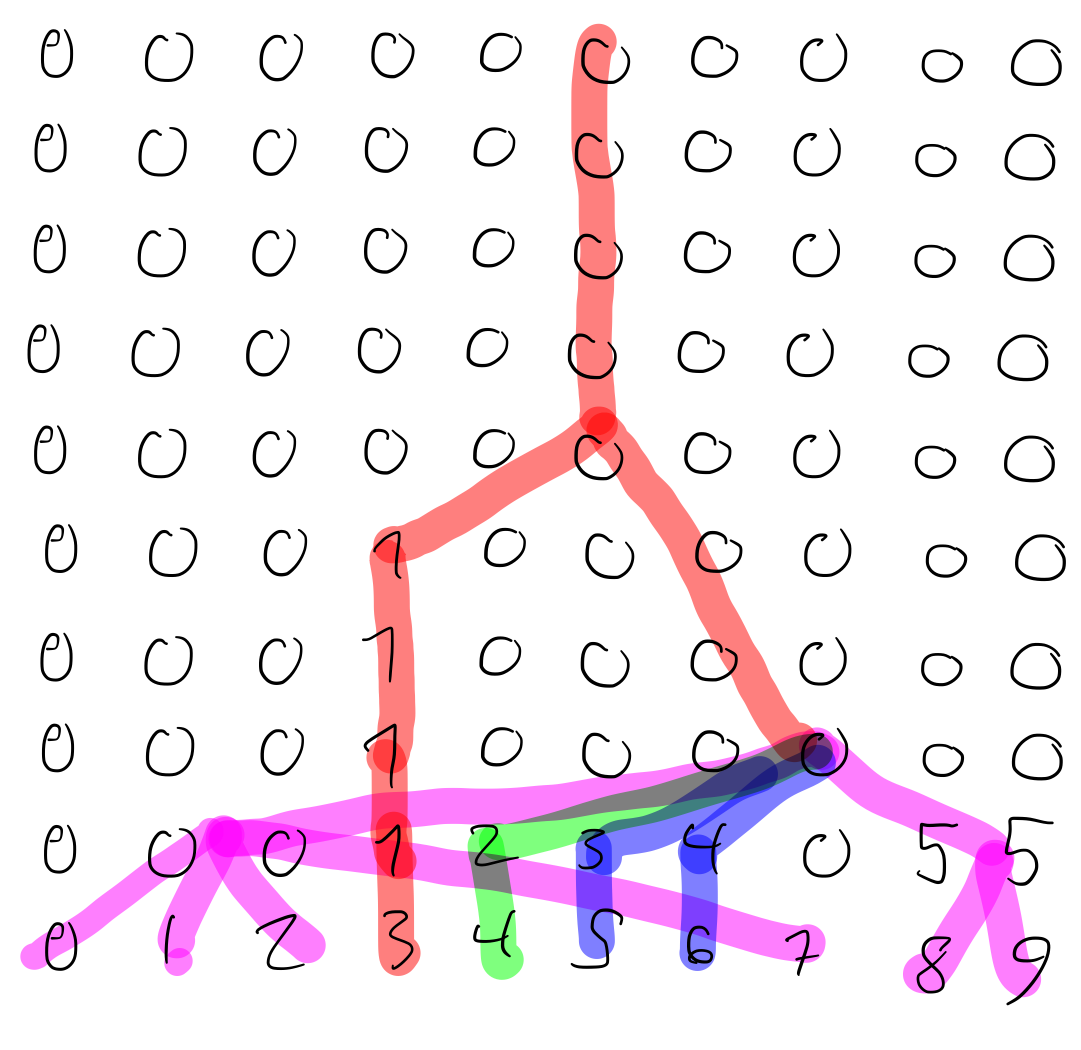
\includegraphics[width=.5\textwidth]{tree}
	\caption{How the tree structure is formed for the connected componenet vectors}
\end{figure}
For example, say $N=8$ and we have
\begin{align*}
c(A^{(j)})=\{0, 0, 0 ,0, 1 ,1 ,1, 1\}\\
c(A^{(j+1)})=\{0, 0, 0 ,0, 1 ,1 ,2, 2\}
\end{align*}
This means that $A^{(j)}$ has two connected components, ordered 0 (with vertices 1,2,3,4) and 1 (with vertices 5,6,7,8) and that $A^{(j+1)}$ has three connected components, ordered 0 (with vertices 1,2,3,4), 1 (with vertices 5 and 6) and 2 (with vertices 7 and 8).  Thus there is a branch from the connect component 1 in $A^{(j)}$ to the connected componenets 1 and 2 in $A^{(j+1)}$. By greedily repeating this iterative algorithm starting with $A^{(1)}$ \footnote{which has by definition only a single connected component and so $c(A^{(1)})=\{0, \cdots, 0\}$} as the root, we produce the tree of topics. Observe that at this stage, all the leaf nodes correspond to actual topics $t_n$. We formulate the topic vectors for the parent nodes by additive percolating up the tree. That is, for a given parent topic $\tau$ with children $\tau_1, \cdots, \tau_k$ we simply have 
$$\tau =\sum_i \tau_i $$

\subsection{Semi-Supervised NNMF}
In many cases, in addition to  $X \in \mathbb{R}^{n\times m}$ we also have a label matrix $Y \in \mathbb{R}^{n\times k}$, where $k$ is the number of cases and $Y_{i,j}$ is 1 if document $i$ is in class $j$ and 0 otherwise. When the data is labeled in this way, we can incorporate this information into the NNMF model to learn a more robust representation of the data.  This \emph{semi-supervised} NNMF  learns a one-versus all separating hyperplane for the observations \cite{lee2010semi}.
Given $B \in \mathbb{R}^{k \times r}$, a basis matrix for $Y$, and $L \in \mathbb{R}^{k \times n}$, a weight matrix to handle missing labels, then the energy function for SSNMF is as follows
$$E - ||(X-AS)||^2 + \lambda ||L \circ (Y-BS)||^2$$
where $\lambda$ is a tradeoff parameter that governs the importance of the supervised term.

In the same vein of Algorithm 1, this energy function yields a convex optimization problem solved by the following algorithm. 

\begin{algorithm}[H]
	\KwIn{k=0; Initialize $A^0, S^0, B^0$}
	\Repeat{Stopping condition}{
		\begin{align*}
		A^{k+1} &= A^k \circ \frac{XS^k}{A^k(S^k)^TS^k}\\
		B^{k+1} &= B^k \circ \frac{(L \circ Y )S^k}{(L \circ B(S^k)^T)S^k}\\
		S^{k+1} &= S^k \circ \frac{(A^{k+1})^TX + \lambda B^T (L \circ Y)}{(A^{k+1})^TAS + \lambda B^T (L \circ BS)}\\
		k &= k+1
		\end{align*} 
	}
	\caption{Multiplicative Update for Semi-Supervised NNMF}
\end{algorithm}
\subsection{Deep Semi NMF}
Semi-Supervised NNMF as discussed above can be thought of as representing $A$ in a low dimensional representation as $S$. In this framework, $A$ is the function that maps the low dimensional representation to the original high dimensional representation. However, as the data becomes increasingly complex, it may have many hierarchy of attributes, each of which requires its own mappings. With the motivation in mind, Trigeorgis et al put forward the notion of a Demi-Smi NNMF \cite{trigeorgis2014deep}.
$$X \approx A_1A_2 \cdots A_m S_m$$
This representation of the data can be achieved by recursively factorizing the low-dimensional representation at each level \cite{trigeorgis2014deep}.
\begin{align*}
S_{m-1} = A_mS_m\\
\vdots \\
S_2  \approx A_3 \cdots A_m  S_m\\
S_1  \approx A_2 \cdots A_m  S_m
\end{align*}

We then consider the algorithms and notions in the domain of Deep Semi NMF as a model for Hierarchical NMF \cite{ deepNonNeg, trigeorgis2014deep} 


\section{Visualization}
I use the d3.js Sunburst implementation to visualize the hierarchical topic model. Arcs at the same level represent discrete topics. A topic on an inner layer that encompasses multiple outer topics represent a super-topic. For example, in Figure 3, the two outer green topics that represent European banking and Chinese banking representatively (with top words$$ \{\text{banks, loans, collateral, abs, ecb bank, lending, small, european, asset}\} $$and $$\{\text{china, economic, reforms, growth, beijing, economy, said, li, year, urged}\}) $$merge into the inner super topic with top words$$ \{\text{banks, china, economic, abs, reforms, growth, loans, collateral, said, beijing}\}.$$

The visualization is responsive, dynamic and available at \\ \texttt{http://www1.cmc.edu/pages/faculty/BHunter/ziv.html}

Next, I extended this visualization to the Semi-Supervised domain using the Afghan Dataset. Here each document has associated with it a class $C\in \{1,\cdots,k\}$ which in this case $k=3$. Recall that the matrix $B \in \mathbb{R}^{k \times r}$ in the semi-supervised NMF model is multiplied by $S$ to obtain an approximation for $Y$, the label matrix. Thus the $i,j$th entry of $B$ can be interpreted in the weighted importance of topic $i$ in predicting class $j$. Thus I sum over the columns of $B$ to capture how important topic $i$ is predicting classes in general. After normalizing, we get a color value $c_i$ for topic $i$, such that
$$c_i = \sum_j B_{i,j} /  \sum_{i,j} B_{i,j}$$
where $c_i=1$ corresponds to yellow and $c_i=0$ corresponds to blue (see Figure 3 right)
\begin{figure}
	\centering
	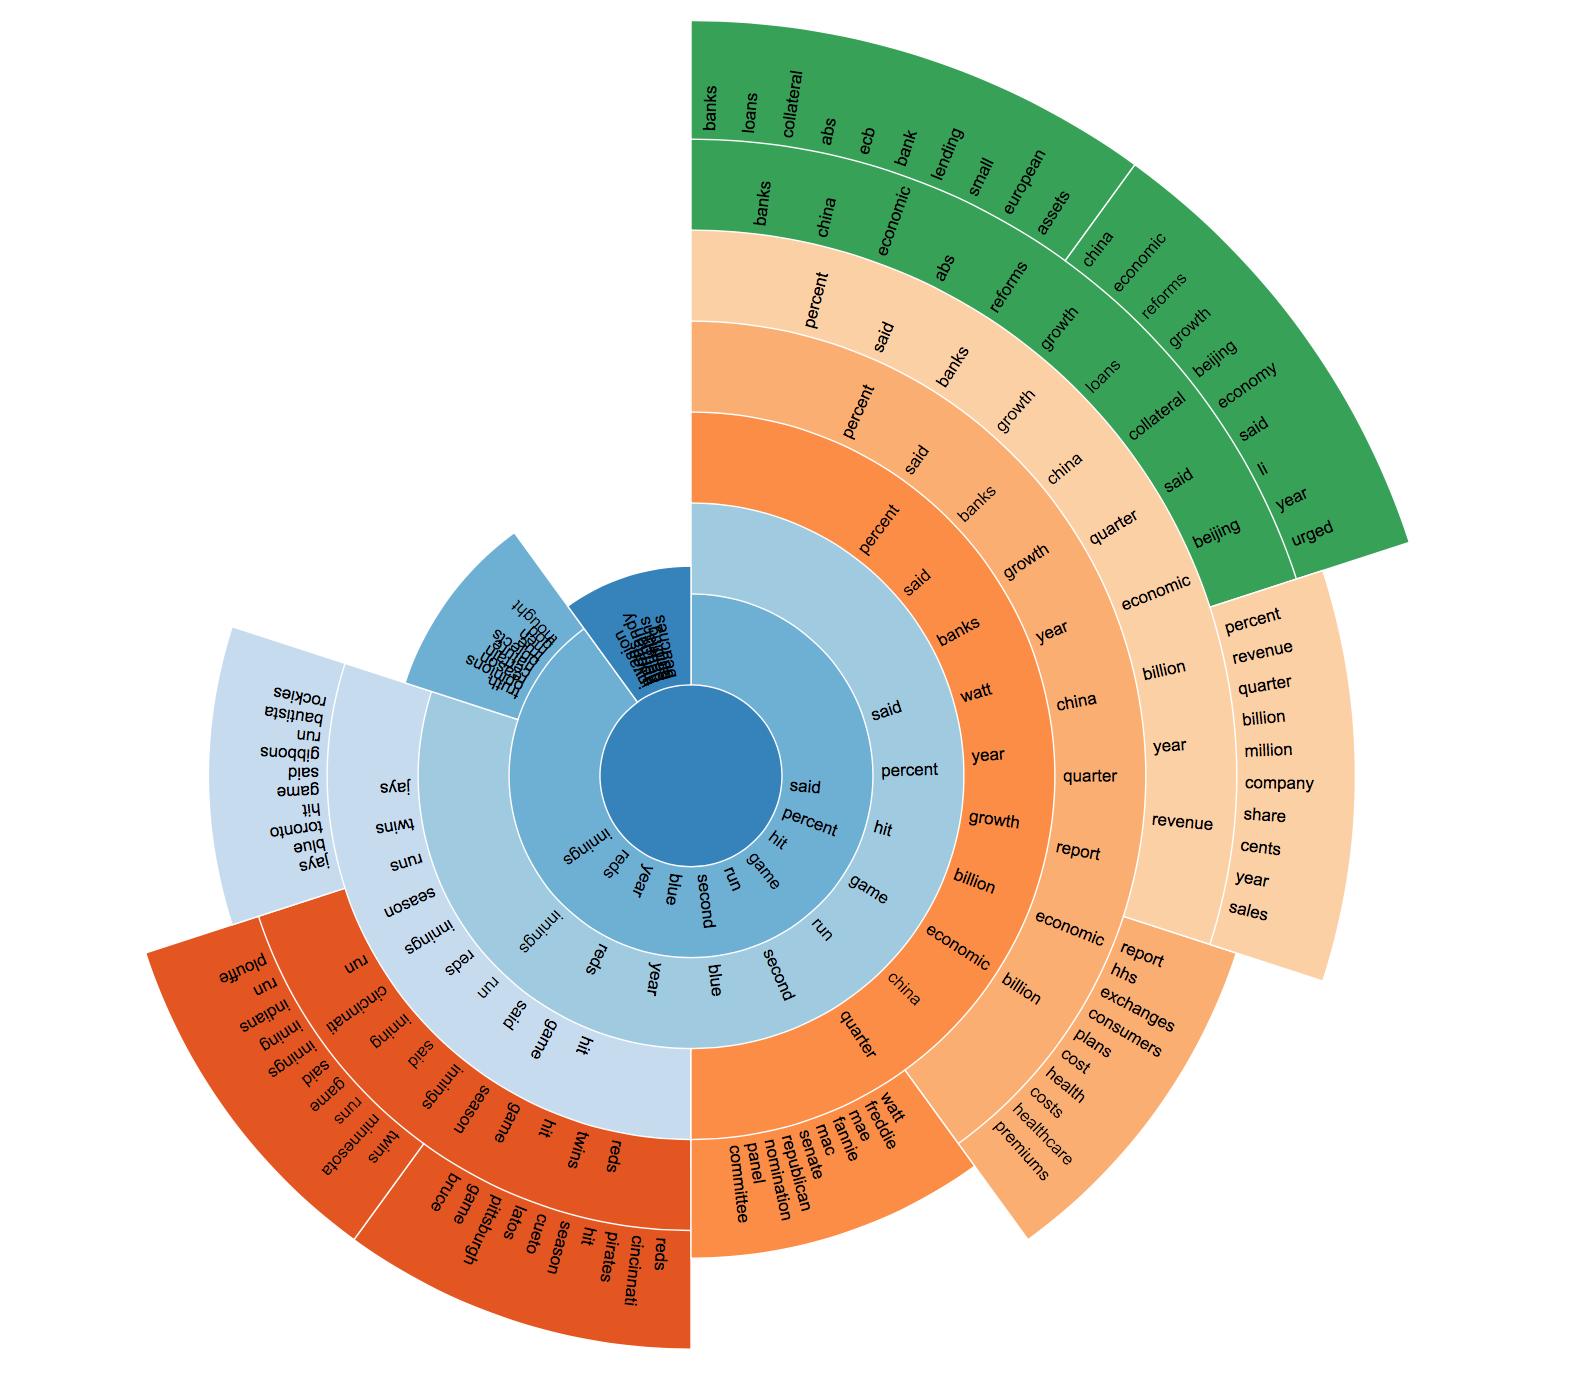
\includegraphics[width=.48\textwidth]{img}
	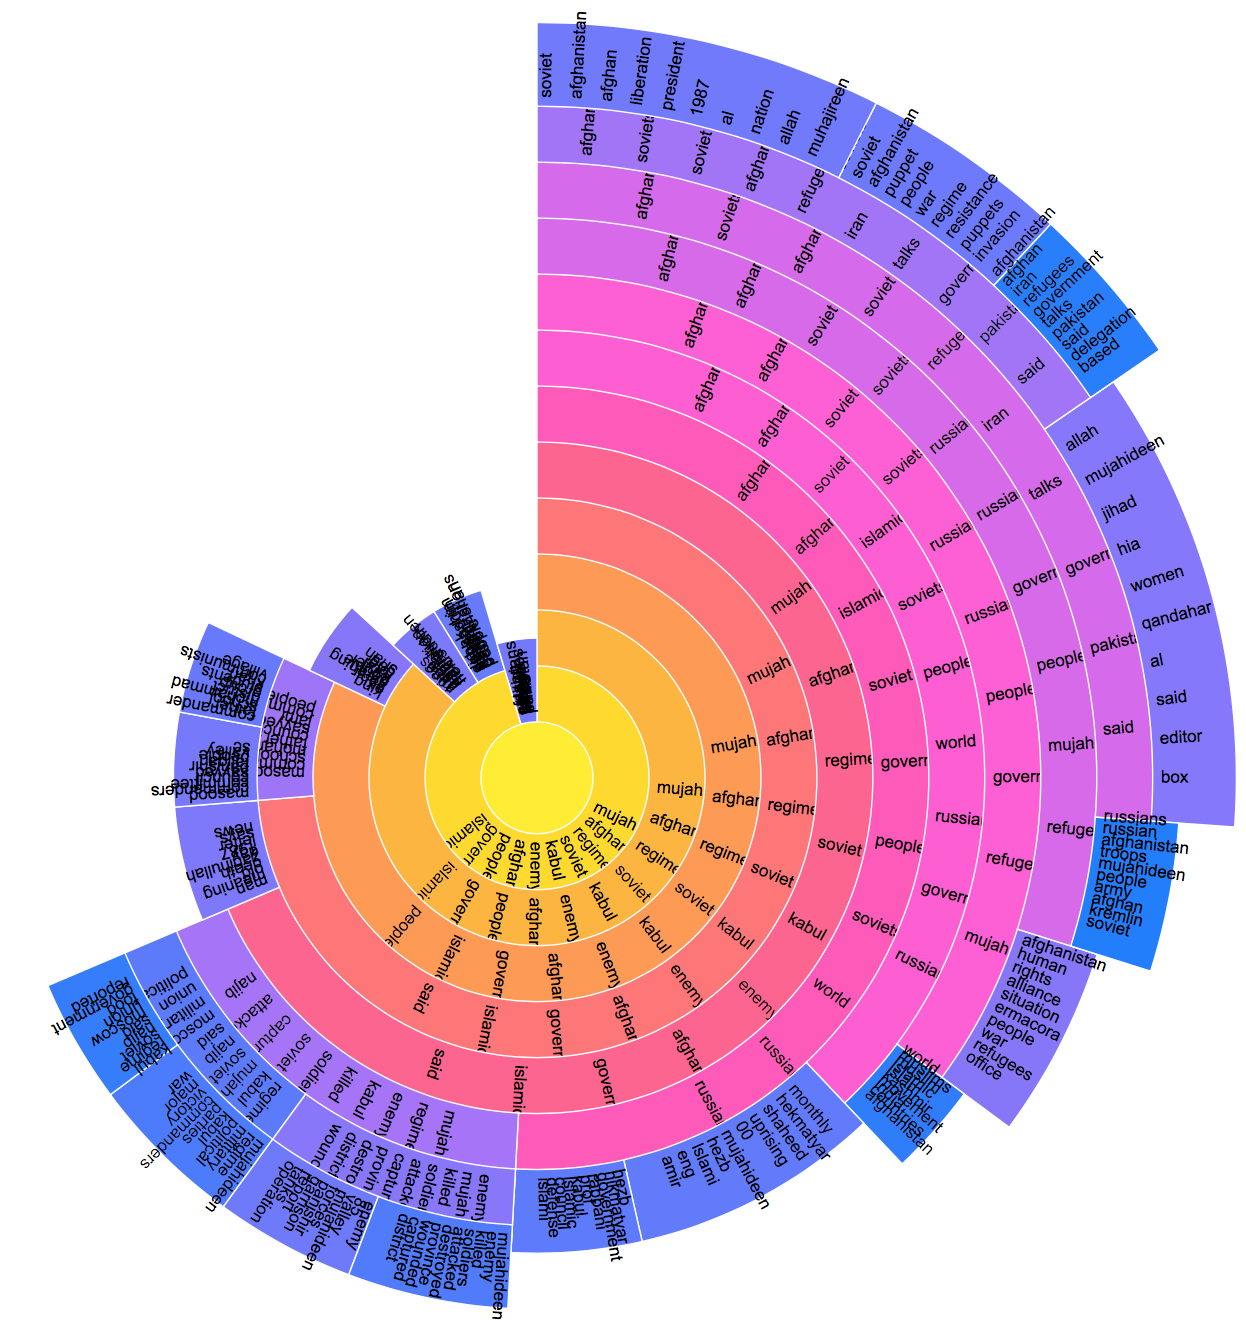
\includegraphics[width=.48\textwidth]{img2}
	\caption{Left: Visualization of hierarchical topics in standard NMF; Right: Visualization of hierarchical topics in  SSNMF; }
\end{figure}

\section{Hierarchical Topic Model}
We will then construct our own model for learning a hierarchy of topics within the model itself. This will be a blend of the Single Linkage graph construction model and the Deep Semi NMF.

\section{Results}
We will then apply the method of our Hierarchical Topic Model to several datasets, and compare our results with previous work.
\subsection{Synthetic Data}
We will generate synthetic data with hierarchical topics and verify that our algorithm succesfully extracts them
\subsection{Standard Data}
We will run our algorithm on data cannonically associated with this task. For our purposes, the 20 News Group Data set will probably be sufficient.
\subsection{Afghan Data}
A collaborator at NYU Abu-Dhabi has hand-curated a dataset of Afghani magazines, which is notable for sociologists. We will run our algorithm on this data set and see what happens

\section{Discussion/Conlusion}
Here we will conclude by situating this work within the field, compare its results with similar methods and propose future work.

\bibliographystyle{plain}

\bibliography{myBib}


\end{document}